\documentclass[answers]{exam}
\usepackage{../HT2025}
\usepackage{graphicx}
\graphicspath{ {./images/} }

\title{Statistics -- Sheet 1\\Asymptotic variance, Q-Q plots}
\author{YOUR NAME HERE :)}
\date{Hilary Term 2025}
% version uploaded 2025-01-06


\begin{document}
\maketitle

\begin{questions}

\question%1
\begin{parts}
\part%1a
Suppose $X_{1}, \ldots, X_{n}$ are independent $\operatorname{Bernoulli}(p)$ random variables. Use the delta method to find the asymptotic distribution of $\widehat{p} /(1-\widehat{p})$ where $\widehat{p}$ is the maximum likelihood estimator of $p$. (The quantity $p /(1-p)$ is the odds of a success.)

\part%1b
Suppose $X_{1}, \ldots, X_{n}$ are independent $\operatorname{Poisson}(\lambda)$ random variables. Find a function $g(\bar{X})$ such that the asymptotic variance of $g(\bar{X})$ does not depend on $\lambda$.
\end{parts}



\question%2
Let $X_{1}, \ldots, X_{n}$ be a random sample from a uniform distribution with probability density function \[
	f(x)= \begin{cases}
		1 & \text{if } 0<x<1 \\
		0 & \text{otherwise.}
	\end{cases}
\]
\begin{parts}
\part%2a
Show that if $X_{(r)}$ is the $r^{\mathrm{th}}$ order statistic, then \[
	E(X_{(r)})=\frac{r}{n+1}, \qquad
	\operatorname{var}(X_{(r)})=\frac{r}{(n+1)(n+2)}\left(1-\frac{r}{n+1}\right).
\] 

\part%2b
Define the median of the random sample, distinguishing between the two cases $n$ odd and $n$ even. Show that the median has expected value $\frac{1}{2}$ if the random sample is drawn from a uniform distribution on $(0,1)$. Find its variance in the case when $n$ is odd. What is the expected value of the median if the random sample is drawn from a uniform distribution on $(a, b)$?
\end{parts}



\question%3
\begin{parts}
\part%3a
Let $X$ be a continuous random variable with cumulative distribution function $F$ which is strictly increasing. If $Y=F(X)$, show that $Y$ is uniformly distributed on the interval $(0,1)$.

\part%3b
The Weibull distribution with parameters $\alpha>0$ and $\lambda>0$ has cumulative distribution function \[
	F(x)= \begin{cases}
		0 & \text{if } x<0, \\
		1-\exp \left(-(x / \lambda)^{\alpha}\right) & \text{if } x \geqslant 0.
	\end{cases}
\] Explain why a probability plot for the Weibull distribution may be based on plotting the logarithm of the $r$th order statistic against $\log \left[-\log \left(1-\frac{r}{n+1}\right)\right]$ and give the slope and intercept of such a plot.
\end{parts}



\question%4
\begin{parts}
\part%4a
Find the expected information for $\theta$, where $0<\theta<1$, based on a random sample $X_{1}, \ldots, X_{n}$ from:
\begin{subparts}
\subpart%4ai
the geometric distribution $f(x ; \theta)=\theta(1-\theta)^{x-1}$, $x=1,2, \ldots$;

\subpart%4aii
the Bernoulli distribution $f(x ; \theta)=\theta^{x}(1-\theta)^{1-x}$, $x=0,1$.
\end{subparts}

\part%4b
A statistician has a choice between observing random samples from the geometric or Bernoulli distributions with the same $\theta$. Which will give the more precise inference about $\theta$?
\end{parts}



\question%5
Suppose a random sample $Y_{1}, \ldots, Y_{n}$ from an exponential distribution with parameter $\lambda$ is rounded down to the nearest $\delta$, giving $Z_{1}, \ldots, Z_{n}$ where $Z_{j}=\delta\left\lfloor\frac{Y_{j}}{\delta}\right\rfloor$.
\begin{parts}
\part%5a
Show that the likelihood contribution from the $j$th rounded observation can be written $(1-e^{-\lambda \delta}) e^{-\lambda z_{j}}$, and deduce that the expected information for $\lambda$ based on the entire sample is \[
	\frac{n \delta^{2} e^{-\lambda \delta}}{(1-e^{-\lambda \delta})^{2}}.
\]

\part%5b
Show that this has limit $n / \lambda^{2}$ as $\delta \to 0$, and that if $\lambda=1$, the loss of information when data are rounded down to the nearest integer rather than recorded exactly, is less than $10 \%$. Find the loss of information when $\delta=0.1$, and comment briefly.
\end{parts}



\question%6
When $T_{1}$ and $T_{2}$ are estimators of a parameter $\theta$, the \emph{asymptotic efficiency} of $T_{1}$ relative to $T_{2}$ is given by $\lim_{n \to \infty} \operatorname{avar}\left(T_{2}\right) / \operatorname{avar}\left(T_{1}\right)$, where $\operatorname{avar}\left(T_{j}\right)$ denotes the asymptotic variance of the approximating normal distribution of $T_{j}, j=1,2$.\\ Suppose $X_{1}, \ldots, X_{n}$ are independent and exponential with parameter $\theta$. Let $\# A$ denote the number of elements of a set $A$, and consider the two estimators \[
	\widetilde{p}=\frac{\#\left\{i: X_{i} \geqslant 1\right\}}{n}\quad
	\text{and}\quad
	\widehat{p}=\bar{X}.
\]
\begin{parts}
\part%6a
Find the asymptotic efficiency of $T_{1}=-\log \widetilde{p}$ relative to $T_{2}=1 / \widehat{p}$.

\part%6b
Find the numerical value of the asymptotic efficiency when $\theta=0.6,1.6,5.6$.

\part%6c
Comment on the implications for using $T_{1}$ instead of $T_{2}$ to estimate $\theta$.
\end{parts}



\question%7
The figure below shows normal Q-Q plots for randomly generated samples of size 100 from four different densities: from a $N(0,1)$ density, an exponential density, a uniform density, and a Cauchy density. (The Cauchy density is $f(x)=[\pi(1+x^{2})]^{-1}$ for $x \in \mathbb{R}$.) Which Q-Q plot goes with which density?
\begin{center}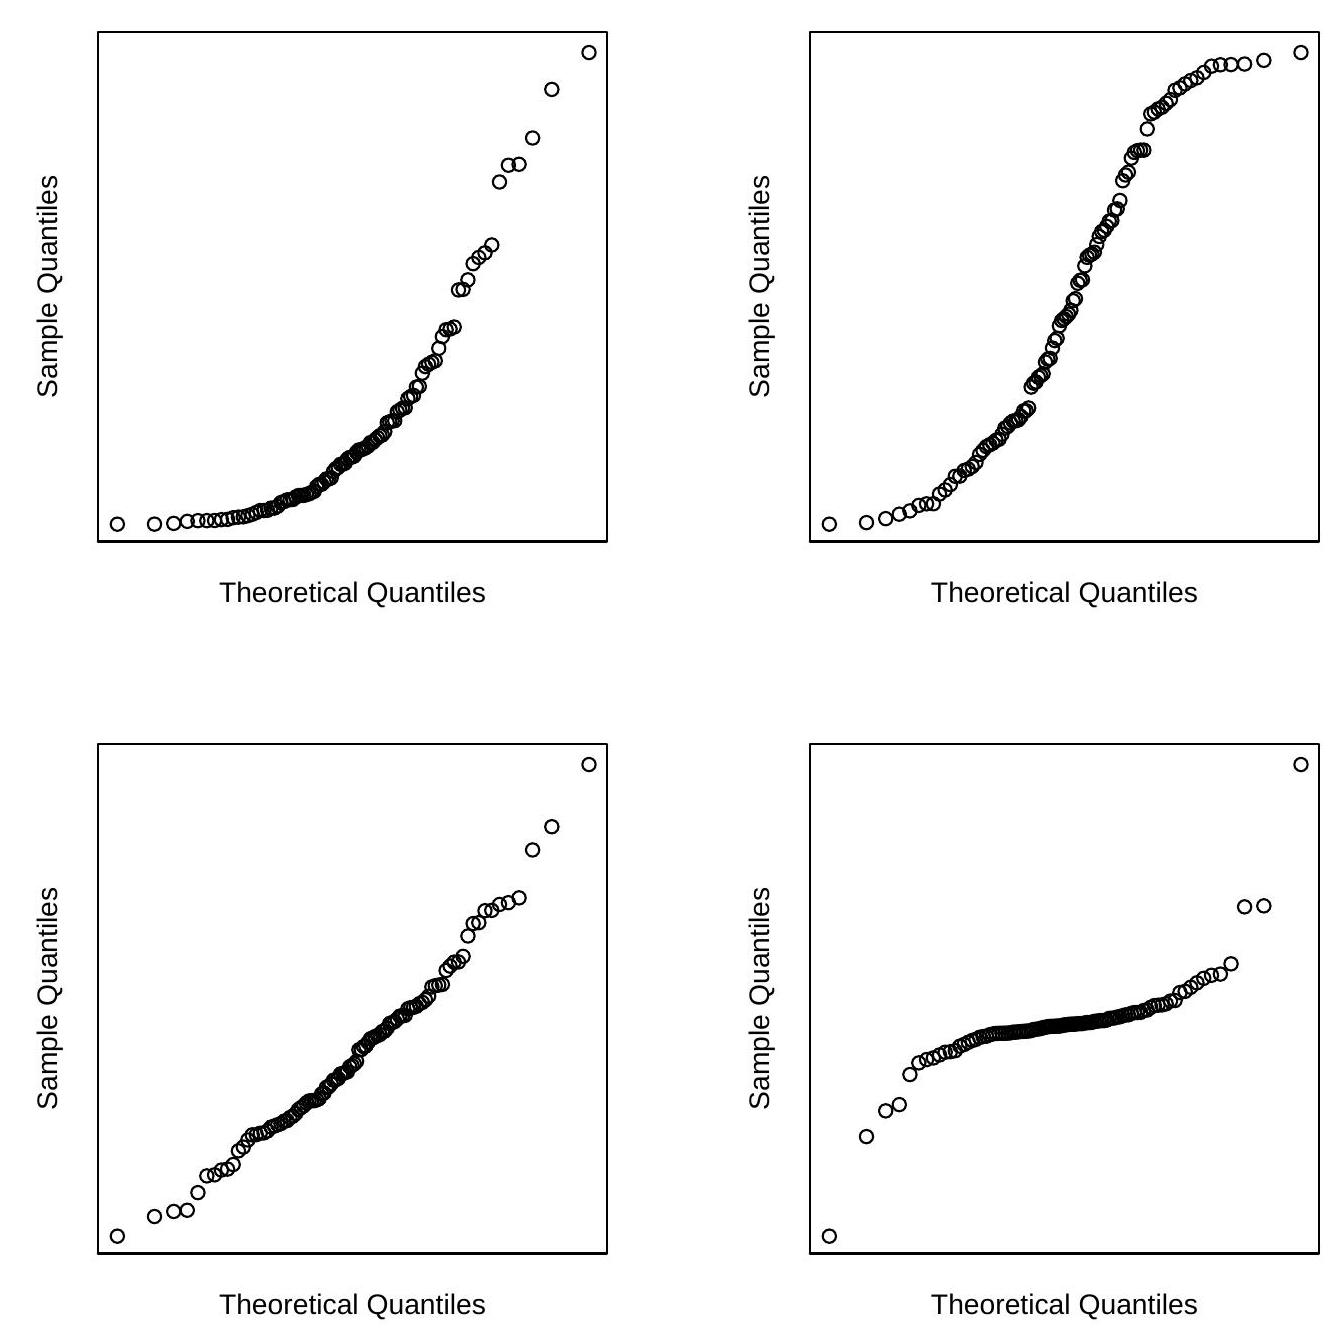
\includegraphics[width=10cm]{sheet 1 q 7}\end{center}



\question%8
Read through the \emph{Getting started with $R$} document (on Moodle) and install R/RStudio and run the commands in the document yourself. The R questions on these problem sheets need only a very small knowledge of R . R code will be supplied in questions and/or at the end of the sheet --- this will be code you can copy and paste into R.\\ Use the R code at the end of the sheet to investigate:
\begin{parts}
\part%8a
How typical is each of the Q-Q plots shown in Figure 1 above? Note that each time we generate a sample (e.g. using \verb|rnorm|, \verb|rexp|, ...) we get a different sample, so we can investigate how typical each one is by doing repeated Q-Q plots.

\part%8b
How much does Figure 1 change if the sample size is smaller (or larger) than 100?
\end{parts}



\question%9
(See the code at the end of this sheet for more.) To generate a sample of size 100 from a $N(0,1)$ density and compare the sample with an exponential distribution, try the following: \begin{verbatim}
n <- 100
x <- rnorm(n)
k <- 1:n
plot(-log(1 - k/(n+1)), sort(x), main = "Exponential Q-Q Plot",
    ylab = "Ordered data", xlab = "-log[1 - k/(n+1)]")
\end{verbatim}
\begin{parts}
\part%9a
Can you explain the shape of this exponential Q-Q plot? What happens (and why) if you repeat but with the line \verb|x <- rnorm(n)| replaced by \verb|x <- rexp(n)|?

\part%9b
Try repeating using the data on insurance claim interarrival times: \begin{verbatim}
x <- scan("http://www.stats.ox.ac.uk/~laws/partA-stats/data/interarrivals.txt")
n <- length(x)
k <- 1:n
\end{verbatim} followed by the plot command above. Try also using the data on insurance claim amounts: \begin{verbatim}
x <- scan("http://www.stats.ox.ac.uk/~laws/partA-stats/data/amounts.txt")
n <- length(x)
k <- 1:n
\end{verbatim} Can you also do a Pareto Q-Q plot for each dataset? What do you conclude?
\end{parts}

\end{questions}

\begin{verbatim}
#### Question 8
# to do one example plot for each distribution in question 7:
x1 <- rnorm(100)
qqnorm(x1)

x2 <- rexp(100)
qqnorm(x2)

x3 <- runif(100)
qqnorm(x3)

# the Cauchy distribution is the t-distribution with 1 degree of freedom
x4 <- rt(100, df = 1)
qqnorm(x4)

# to see all four plots at once in a 2 x 2 array
# use par(mfrow = c(2, 2)) and then the qqnorm commands
par(mfrow = c(2, 2))
# from now on plots will be in a 2 x 2 array

x1 <- rnorm(100)
qqnorm(x1, main = "Normal Q-Q plot: normal data")

x2 <- rexp(100)
qqnorm(x2, main = "Normal Q-Q plot: exponential data")

x3 <- runif(100)
qqnorm(x3, main = "Normal Q-Q plot: uniform data")

x4 <- rt(100, df = 1)
qqnorm(x4, main = "Normal Q-Q plot: Cauchy data")

# to get back to a 1 x 1 array of plots you would use
# par(mfrow = c(1, 1))

# try multiple plots to see how much variation there is
# from one sample to another
# normal data, n = 100, try running this a few times
for (i in 1:4) {
    x <- rnorm(100)
    qqnorm(x)
}

# and repeat but with x <- rexp(100)
# and with x <- runif(100)
# and with x <- rt(100, df = 1)

# next, vary the sample size
# normal data, n = 10
for (i in 1:4) {
    x <- rnorm(10)
    qqnorm(x)
}

# useful to also try n = 20, 50
# useful to also try exponential data (using rexp),
# and uniform data (using runif),
# and Cauchy, or t, data (using rt)

# e.g. uniform distribution, n = 20
for (i in 1:4) {
    x <- runif(20)
    qqnorm(x)
}

# can also look at t-distributions with different numbers
# of degrees of freedom
# e.g. t-distribution with 5 degrees of freedom, n = 10
for (i in 1:4) {
    x <- rt(10, df = 5)
    qqnorm(x)
}

#### Question 9
n <- 100
x <- rnorm(n)
k <- 1:n
plot(-log(1 - k/(n+1)), sort(x), main = "Exponential Q-Q Plot",
    ylab = "Ordered data", xlab = "-log[1 - k/(n+1)]")

# now try replacing x <- rnorm(n) by x <- rexp(n)
x <- rexp(n)
plot(-log(1 - k/(n+1)), sort(x), main = "Exponential Q-Q Plot",
    ylab = "Ordered data", xlab = "-log[1 - k/(n+1)]")

# are interarrival times exponential?
# exponential Q-Q plot with data on insurance claim interarrival times
x <- scan("http://www.stats.ox.ac.uk/~laws/partA-stats/data/interarrivals.txt")
n <- length(x)
k <- 1:n
plot(-log(1 - k/(n+1)), sort(x), main = "Exponential Q-Q Plot",
    ylab = "Ordered data", xlab = "-log[1 - k/(n+1)]")

# are claim amounts exponential?
# exponential Q-Q plot with data on insurance claim amounts
x <- scan("http://www.stats.ox.ac.uk/~laws/partA-stats/data/amounts.txt")
n <- length(x)
k <- 1:n
plot(-log(1 - k/(n+1)), sort(x), main = "Exponential Q-Q Plot",
    ylab = "Ordered data", xlab = "-log[1 - k/(n+1)]")

# are interarrival times Pareto?
# Pareto Q-Q plot for interarrival times
x <- scan("http://www.stats.ox.ac.uk/~laws/partA-stats/data/interarrivals.txt")
n <- length(x)
k <- 1:n
plot(-log(1 - k/(n+1)), sort(log(x)),
    main = "Pareto Q-Q Plot: interarrivals",
    ylab = "log(Ordered data)", xlab = "-log[1 - k/(n+1)]")

# are claim amounts Pareto?
# Pareto Q-Q plot for claim amounts
x <- scan("http://www.stats.ox.ac.uk/~laws/partA-stats/data/amounts.txt")
n <- length(x)
k <- 1:n
plot(-log(1 - k/(n+1)), sort(log(x)),
    main = "Pareto Q-Q Plot: amounts",
    ylab = "log(Ordered data)", xlab = "-log[1 - k/(n+1)]")
\end{verbatim}

\end{document}
